\documentclass[tikz,border=8pt]{standalone}
% Shared look for every TikZ diagram. Load with \input{../../tools/tikz-style.tex}
\usepackage[sfdefault]{roboto}
\usetikzlibrary{arrows.meta, positioning, shapes.geometric, calc, fit, backgrounds}
\definecolor{cblue}{HTML}{4C78A8}
\definecolor{corange}{HTML}{F58518}
\definecolor{cgreen}{HTML}{54A24B}
\definecolor{cred}{HTML}{E45756}
\definecolor{cpurple}{HTML}{B279A2}
\definecolor{cgrey}{HTML}{6B6B6B}
\tikzset{
  every picture/.style={font=\sffamily, line width=1.2pt},
  box/.style={draw=#1, fill=#1!12, rounded corners=4pt, align=center, inner sep=7pt, minimum height=1.1cm},
  box/.default=cgrey,
  arrow/.style={-{Stealth[length=3mm]}, draw=cgrey, line width=1.4pt},
  title/.style={font=\sffamily\bfseries\Large},
  note/.style={font=\sffamily\small, text=cgrey, align=center},
}
\AtBeginDocument{\hyphenpenalty=10000 \exhyphenpenalty=10000}

% The room robot's stack (RO-075) as ROS 2 nodes: ovals are nodes (programs), boxes are topics, the dashed arrows a
% service (request and reply) and an action (goal, feedback, result). Rates: scan every 0.1 s (a scanner like the
% Hokuyo URG-04LX-UG01), odometry and commands every 0.05 s, local plan every 0.1 s.
\begin{document}
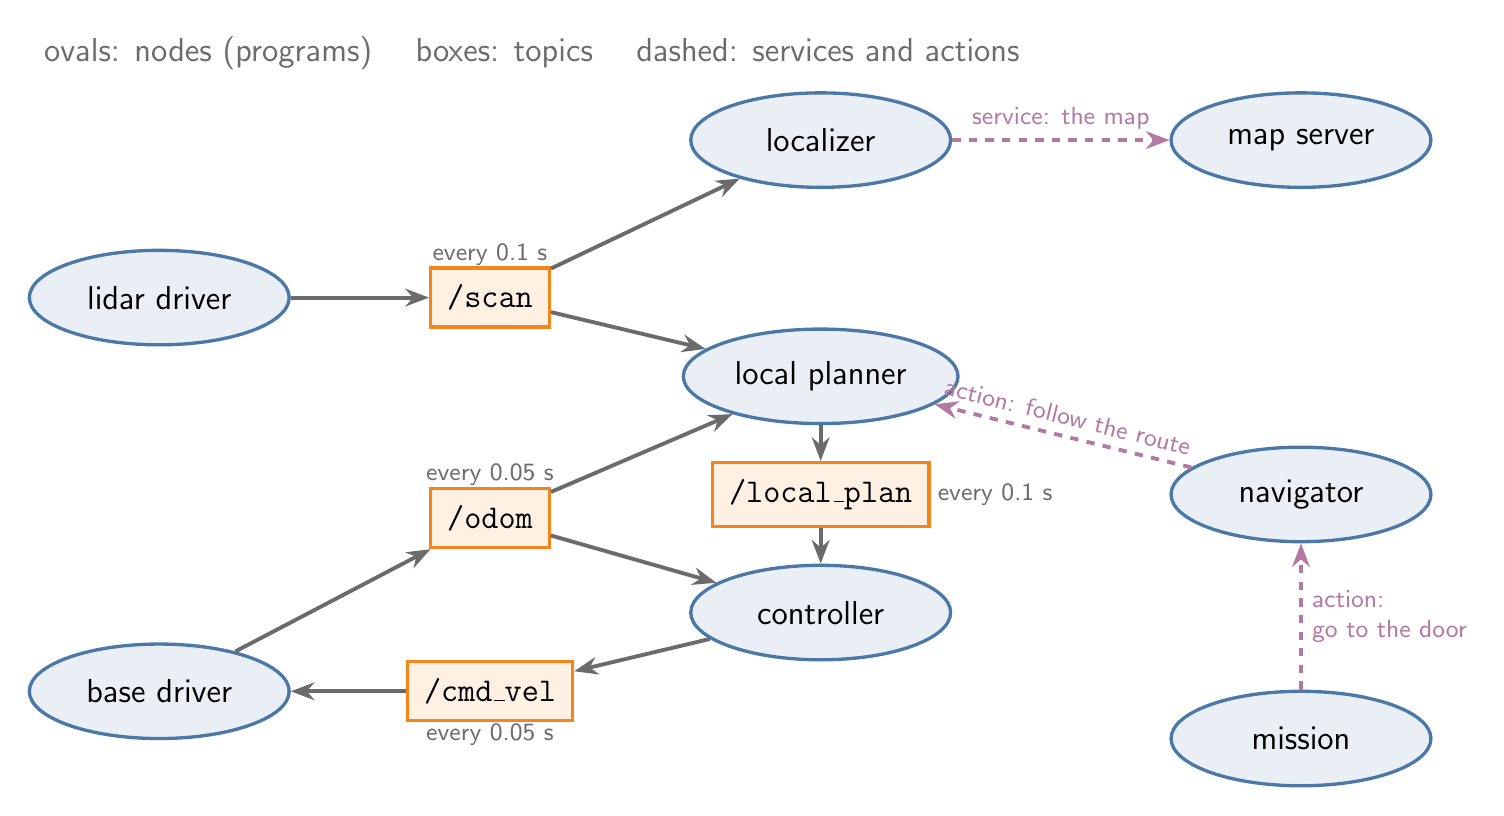
\begin{tikzpicture}[
  nd/.style={draw=cblue, fill=cblue!12, ellipse, font=\sffamily\large, inner sep=4pt, minimum width=3.3cm, minimum height=1.2cm},
  tp/.style={draw=corange, fill=corange!12, rectangle, font=\ttfamily\large, inner sep=6pt},
  ar/.style={-{Stealth[length=3mm]}, draw=cgrey, line width=1.4pt},
  sv/.style={-{Stealth[length=3mm]}, draw=cpurple, line width=1.4pt, dashed}]
  \node[nd] (lidar) at (0,4) {lidar driver};
  \node[nd] (base) at (0,-1) {base driver};
  \node[nd] (loc) at (8.4,6) {localizer};
  \node[nd] (lp) at (8.4,3) {local planner};
  \node[nd] (ctl) at (8.4,0) {controller};
  \node[nd] (map) at (14.5,6) {map server};
  \node[nd] (nav) at (14.5,1.5) {navigator};
  \node[nd] (mis) at (14.5,-1.6) {mission};
  \node[tp] (scan) at (4.2,4) {/scan};
  \node[tp] (odom) at (4.2,1.2) {/odom};
  \node[tp] (plan) at (8.4,1.5) {/local\_plan};
  \node[tp] (cmd) at (4.2,-1) {/cmd\_vel};
  \draw[ar] (lidar) -- (scan); \draw[ar] (scan) -- (loc); \draw[ar] (scan) -- (lp);
  \draw[ar] (base) -- (odom); \draw[ar] (odom) -- (lp); \draw[ar] (odom) -- (ctl);
  \draw[ar] (lp) -- (plan); \draw[ar] (plan) -- (ctl);
  \draw[ar] (ctl) -- (cmd); \draw[ar] (cmd) -- (base);
  \draw[sv] (loc.east) -- node[note, above, text=cpurple] {service: the map} (map.west);
  \draw[sv] (mis) -- node[note, right, text=cpurple, align=left] {action:\\ go to the door} (nav);
  \draw[sv] (nav) -- node[note, above, text=cpurple, align=center, sloped] {action: follow the route} (lp);
  \node[note, font=\sffamily\small] at (4.2,4.55) {every 0.1 s};
  \node[note, font=\sffamily\small] at (4.2,1.75) {every 0.05 s};
  \node[note, font=\sffamily\small, anchor=west] at (9.75,1.5) {every 0.1 s};
  \node[note, font=\sffamily\small] at (4.2,-1.55) {every 0.05 s};
  \node[note, font=\sffamily\large, anchor=west] at (-1.6,7.1) {ovals: nodes (programs) \quad boxes: topics \quad dashed: services and actions};
\end{tikzpicture}
\end{document}
